\section{Detection and Time Synchronization}%
\label{sec:detection}

\begin{figure}[t]
  \centerline{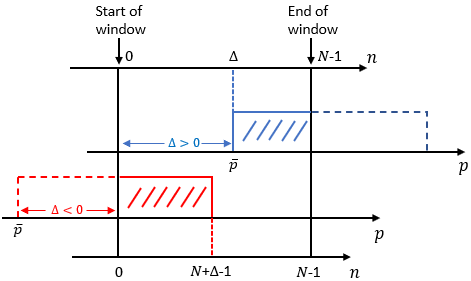
\includegraphics[width=2.75in]{partial_preamble_detection.png}}
  \caption{The current window with local time-scale $n$ may contain a
    partial preamble. The preamble starts at $\bar{p}$ on global scale.
    The start of the preamble relative to the window is $\Delta$. The cases $\Delta >0$ and $\Delta < 0$
    are illustrated.}
  \label{fig:partial_preamble_detection}
  \end{figure}

% In this section, we analyze the sequential detection problem, where 
% the detection algorithm proceeds sequentially and each step a window of
% $N$ received samples with $N{-}1$ overlapped samples from the previous window is considered.
We start by looking at the two hypotheses for the sequential detection task:
Let $H_0$ be the null hypothesis that the received signal is the
channel noise or only contains a portion of the preamble against the
alternative $H_1$ that it contains the entire preamble.  
% The detection algorithm proceeds sequentially and each step a window of
% length $N$ received samples with $N-1$ overlapped samples from the previous window is considered.
Define $\Delta$ to be the distance between the current start position of the window
of $N$ received samples and the start position of the preamble $\bar{p}$.
Figure~\ref{fig:partial_preamble_detection} illustrates two distinct cases when a portion of the 
preamble is in the window.
%with global delay index $p$ and local sample index $n$.
In terms of the local scale $n=0,1,\ldots,N-1$, the two hypotheses are given by the window of samples $r_n$
\begin{equation}
  \label{eq:two hypotheses}
  \begin{aligned}
  &H_0{:}~r_n{=}
  \begin{dcases}
      s_{n-\Delta}\xi e^{j2\pi\delta (n-\Delta)}{+}w_n & \max(0{,}\Delta){\leq} n{<} \min(N{,}N{+}\Delta) \\
      % s_{n-\Delta}\xi e^{j2\pi\delta (n-\Delta)}{+}w_n & n{\in}[\max(0,\Delta), \min(N,N{+}\Delta)) \\
      w_n & \text{otherwise},
  \end{dcases} \\
  &H_1{:}~r_n{=}s_n\xi e^{j2\pi\delta n}+w_n.
  \end{aligned}
\end{equation}
where $\xi=Ae^{j\phi}$ denotes the phasor in~\eqref{eq:model}.
Furthermore, $\Delta \neq 0$ is the premise under hypothesis $H_0$
while $\Delta=0$ under $H_1$.  
% Figure 3 demonstrates the case when $H_0$ represents a portion of the preamble compared with
% $H_1$. 

% In~\cite{Ramakrishnan_10,Chiani_06,Liang_15},
% the authors define hypothesis $H_0$ only when no preamble
% is observed, i.e., $|\Delta| \geq N$. Although, in~\cite{Chiani_06},
% it is pointed out the effect of partial preamble can be neglected by
% using the preamble symbol sequence with a good autocorrelation property.
% In this paper, we still focus on discussing when partial preamble is observed because it is the worst case of $H_0$
% and it affects the result of hypothesis testing.

We focus on discussing when the start of the preamble 
occurs in the window, i.e., $\Delta\in(0,N{-}1]$, which corresponds to
the top case in figure~\ref{fig:partial_preamble_detection}.
The bottom case when 
$\Delta\in[-N{+}1,0)$ 
is symmetric to the top case.
Based on~\eqref{eq:two hypotheses}, we build conditional likelihood ratio test (CLRT)
between $H_0$ and $H_1$ by conditioning on the distance $\Delta$, 
the phasor $\xi$ and the frequency offset $\delta$. The likelihood ratio is given by
\begin{equation}
    \label{eq:likelihood ratio}
    \begin{aligned}
    \Lambda(R|\Delta,\xi,\delta)&=\frac{f_{R|H_1,\xi,\delta}(r|H_1,\xi,\delta)}{f_{R|H_0,\Delta,\xi,\delta}(r|H_1,\Delta,\xi,\delta)} \\
    &=\frac{\displaystyle \prod_{n=0}^{N-1}\frac{1}{\sqrt{\pi N_0}}e^{-\frac{|r_n-s_n\xi e^{j2\pi\delta n}|^2}{N_0}}}{\displaystyle \frac{1}{(\pi N_0)^{N/2}}\prod_{n=\Delta}^{N-1}e^{-\frac{|r_n-s_{n-\Delta}\xi e^{j2\pi\delta (n-\Delta)}|^2}{N_0}}\prod_{n=0}^{\Delta-1}e^{-\frac{|r_n|^2}{N_0}}} \\
    % &=\frac{\prod_{n=0}^{N-1}\frac{1}{\sqrt{\pi N_0}}e^{-\frac{|r_n-s_n\xi e^{j2\pi\delta n}|^2}{N_0}}}{\prod_{n=\Delta}^{N-1}\frac{1}{\sqrt{\pi N_0}}e^{-\frac{|r_n-s_{n-\Delta}\xi e^{j2\pi\delta (n-\Delta)}|^2}{N_0}}\prod_{n=0}^{\Delta-1}\frac{1}{\sqrt{\pi N_0}}e^{-\frac{|r_n|^2}{N_0}}} \\
    % &\times \frac{1}{\prod_{n=0}^{\Delta-1}\frac{1}{\sqrt{\pi N_0}}e^{-\frac{|r_n|^2}{N_0}}}
    & \LRT{H_1}{H_0} \eta.
    \end{aligned}
  \end{equation}

  Canceling the common parts and taking the logarithm,~\eqref{eq:likelihood ratio} is reduced to
\begin{equation}
    \label{eq:log likelihood}
    \begin{aligned}
    \Re\Bigg\{\sum_{n=0}^{N-1}r_ns_n^*\xi^*e^{-j2\pi\delta n}-\sum_{n=\Delta}^{N-1}r_n&s_{n-\Delta}^*\xi^*e^{-j2\pi\delta(n-\Delta)}\Bigg\} \LRT{H_1}{H_0} \\
    &\frac{N_0}{2}\ln\eta+\frac{A^2}{2}\sum_{n=N-\Delta}^{N-1}|s_n|^2.
    \end{aligned}
\end{equation}

On the left hand side, the two summations are the matched filters for hypothesis $H_1$
and $H_0$, respectively. 
It can be shown that the principal value of the left hand side of~\eqref{eq:log likelihood}
reduces to the difference between the energy of the preamble and a partial
autocorrelation function (ACF) of the preamble at lag $\Delta$ under
the two hypotheses.
Moreover, we notice the second summation on the left hand side is not computable
due to the unknown information of $\Delta$ while the first summation is.
On the other hand,
the first summation reflects the energy of the preamble
under $H_1$ and the partial ACF of the preamble at lag $\Delta$ under $H_0$.
To mitigate the effect of the partial ACF a preamble
with very good autocorrelation properties is critical.

Thus, a practical sequential detector reduces to the
cross-correlation between the received signal
and the preamble corrected by the frequency and phasor estimates with
proper scaling.
Specifically, for each window starting at global sample index $p$
\begin{equation}
  \label{eq:generalized_corr}
  \rho(p)=
  \frac{\Re\{\langle
    \bm{r}_{p},\hat{\bm{s}}_{p}\rangle\}}
  {||\bm{r}_{p}||\cdot||\hat{\bm{s}}_{p}||} \LRT{H_1}{H_0} \gamma
\end{equation}
where $\bm{r}_{p}{=}[r_{p},r_{p+1},\ldots,r_{p+N-1}]$ denotes the window of received signal
starting at position $p$. $\hat{\bm{s}}_{p}$ denotes the carrier-corrected preamble,
where each element is $\hat{s}_{n}=s_n\hat{\xi}_{p}e^{j2\pi\hat{\delta}_{p}n}$
for $n=0,1,\ldots,N{-}1$, and $\hat{\xi}_{p}$, $\hat{\delta}_{p}$ are the carrier estimates at
position $p$.
%$||\cdot||$ is the Euclidean norm of the signal sequence, and
$\gamma$ is the normalized detection threshold which lies in the range of $[0,1]$. 
From~\eqref{eq:generalized_corr}, we see
a realistic generalized likelihood ratio test (GLRT) replaces the CLRT
by first performing  carrier estimation of the signal in window at
each position $p$
and then applying corrections based on these estimates in the LRT.\@
It should be emphasized that our detector is intended to work at high sample rate;
While~\eqref{eq:generalized_corr} is straightforward and of complexity 
$O(N)$, the complexity of estimating $\hat{\xi}$,$\hat{\delta}$
is critical for practical implementation.  
A pair of low-complexity frequency and phasor estimates will be given in the next section.


% On the left hand side, the two summations are the matched filters for hypothesis $H_1$
% and $H_0$, respectively. It is easy to derive that the principal value of the log-CLRT
% reduces to the difference between the energy of the (partial) preamble and a partial
% autocorrelation function (ACF) of the preamble at lag $\Delta$ under two hypotheses.

% It can be also seen that the second summation of~\eqref{eq:log likelihood} is not computable
% due to the unknown information of the distance $\Delta$.

% To explain this, we plug $r_n=s_n\xi e^{j2\pi\delta n}+w_n$ under hypothesis $H_1$ into the left hand side of~\eqref{eq:log likelihood}.
% In the real operator, it yields

% \begin{equation}
%     \label{eq:log likelihood under H_1}
%     \begin{aligned}
%     % &\sigma(\Delta) \\    
%     % &=A^2\sum_{n=0}^{N-1}|s_n|^2-A^2e^{j2\pi\delta\Delta}\sum_{n=\Delta}^{N-1}s_ns_{n-\Delta}^*+\text{a zero-mean AWGN}
%     A^2\sum_{n=0}^{N-1}|s_n|^2-A^2e^{j2\pi\delta\Delta}\sum_{n=\Delta}^{N-1}s_ns_{n-\Delta}^*+\text{zero-mean noise},
%     \end{aligned}
% \end{equation}
% where $A^2\sum_{n=0}^{N-1}|s_n|^2$ denotes the energy of the preamble and
% $\sum_{n=\Delta}^{N-1}s_ns_{n-\Delta}^*$ is the partial autocorrelation function (ACF) of the
% preamble at lag $\Delta$. Similarly, it can be derived the left hand side of~\eqref{eq:log likelihood}
% under hypothesis $H_0$ in the real operator is 
% % $-A^2\sum_{n=\Delta}^{N-1}|s_{n-\Delta}|^2+A^2e^{-j2\pi\delta\Delta}\sum_{n=\Delta}^{N-1}s_{n-\Delta}s_n^*$

% \begin{equation}
%     \label{eq:log likelihood under H_0}
%     \begin{aligned}
%     % &\sigma(\Delta) \\    
%     % &=A^2\sum_{n=0}^{N-1}|s_n|^2-A^2e^{j2\pi\delta\Delta}\sum_{n=\Delta}^{N-1}s_ns_{n-\Delta}^*+\text{a zero-mean AWGN}
%     -A^2\sum_{n=\Delta}^{N-1}|s_{n-\Delta}|^2+A^2e^{-j2\pi\delta\Delta}\sum_{n=\Delta}^{N-1}s_{n-\Delta}s_n^*+\text{zero-mean noise}.
%     \end{aligned}
% \end{equation}
% Thus, based on~\eqref{eq:log likelihood under H_1} and~\eqref{eq:log likelihood under H_0},
% we can conclude that the principle value of the log-CLRT reduces to the difference between
% the energy of the (partial) preamble and the ACF of the preamble sequence at lag $\Delta$. 
% By using the symbol sequence $\{c_i\}$ of $s_n$ with a good autocorrelation property, e.g., Gold sequence, the
% effect of the ACF can be kindly mitigated; However, because of pulse shaping,
% the autocorrelation property of the preamble is decreased so that 
% the effect of the ACF cannot be ignored. 

% In practice, the distance $\Delta$ is an unknown information to the receiver,
% which means the second summation of~\eqref{eq:log likelihood} is not computable.
% However, the first summation is computable and it reflects the energy of the preamble under
% $H_1$ and the partial ACF under $H_0$.
% Thus, a practical sequential detector is built just based on the classical 
% cross-correlation between the received signal
% and the preamble corrected by the frequency and phasor estimates with some proper scaling. Specifically,

% \begin{equation}
%     \label{eq:generalized_corr}
%     \rho(\tilde{p})=
%     \frac{\Re\{\langle
%       \bm{r}_{\tilde{p}},\hat{\bm{s}}_{\tilde{p}}\rangle\}}
%     {||\bm{r}_{\tilde{p}}||\cdot||\hat{\bm{s}}_{\tilde{p}}||} \LRT{H_1}{H_0} \gamma
%   \end{equation}
% where $\tilde{p}{=}p{+}\Delta$ denotes the general start position of received signal. 
% $\bm{r}_{\tilde{p}}{=}[r_{\tilde{p}},r_{\tilde{p}+1},\ldots,r_{\tilde{p}+N-1}]$ represents the received signal sequence at
% the position $\tilde{p}$, and $\hat{\bm{s}}_{\tilde{p}}$ represents the carrier-estimates corrected preamble sequence, where each element is 
% $\hat{s}_{n}=s_n\hat{\xi}_{\tilde{p}}e^{j2\pi\hat{\delta}_{\tilde{p}}n}~\text{for}~n=0,1,\ldots,N-1$, and $\hat{\xi}_{\tilde{p}}$, $\hat{\delta}_{\tilde{p}}$
% are the phasor and frequency estimates at position $\tilde{p}$. Moreover, $||\cdot||$ is the Euclidean norm of the signal sequence,
% and $\gamma$ is the normalized detection threshold which lies on the range of $[0,1]$. 
% From~\eqref{eq:generalized_corr}, it is obvious that to implement the sequential detector, we need the information
% of the frequency and phasor estimates at that position. Thus, 

% a realistic generalized likelihood ratio test (GLRT) replaces the CLRT of~\eqref{eq:likelihood ratio}
% by first doing carrier synchronization at each position of detection then plugging the estimates into the LRT.
% Furthermore, it should be emphasized that our sequential detector requires to work at high sample rate; Although~\eqref{eq:generalized_corr}
% is already the simpliest form, the complexity of the two estimates $\hat{\xi}$,$\hat{\delta}$ is also crucial. 
% A pair of low-complexity frequency and phasor estimates will be given in the next section.





